\section{Solving Linear Programs}
From now on we'll characterize the system of unequations by a matrix and a vector. $A\vec x \geq \vec b$. The objective function can also be written in vector form $\min \vec c \vec x$, where $c$ is the cost vector.

Solving LPs with just two variables is rather easy. We can use a graphical approach in two dimensions. The constraints define halfplanes in the 2D space. The feasible region of the problem is then the intersection of all the halfplanes. The cost vector now defines a halfspace of its own (i.e. lines with equivalent costs) that can be shifted around by choosing different $x$. If $x$ lies within the feasible region we get a feasible solution. The goal is to shift the lines as far in negative $c$ direction as possible without leaving the feasible region. See figure \ref{Fig:graphSolutionEx}.

\begin{figure}[hbt]
\begin{minipage}[hbt]{0.4\linewidth}
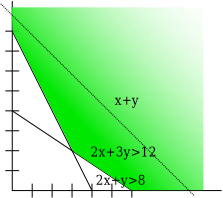
\includegraphics{./images/graphSolutionEx.pdf}
\end{minipage}
\hfill
\begin{minipage}[hbt]{0.4\linewidth}
\begin{align*}
\min x+y\\
2x+y\geq 8\\
2x+3y\geq 12
\end{align*}
\end{minipage}
\caption{An example for a graphical solution of an LP. The optimal solution is (3,2)}
\label{Fig:graphSolutionEx}
\end{figure}

How can we derive an algorithm from this method? We use the idea of silding down, but just look at the corners of the feasible region, to get discrete steps (continuous sliding can't be implemented well). We start with any corner of the feasible region (a basic feasible solution) and look at its neighbours. Should they have a better objective value we move, else we're finished. 

To formalize that we need a notion of a corner in a (usually highdimensional) feasible region. To use it in a program it should be a nongraphical definition. We give three different alternatives and prove that they are all equivalent.

\begin{Def}[Polyhedron] A set in $\R^n$ whose members obey a set of linear inequalitios
\[\{x\in \R^n | Ax \geq b\} \qquad A\in \R^{m\times n},\ b\in \R^m\]
\end{Def}

\begin{Def}[Hyperplane, Hyperspace] \label{Def:hyperPlaneSpace} Let $a\in \R^n$, $a\neq 0$ and a scalar $\lambda \in \R$ 
\begin{enumerate}
\item $\{x|ax=b\}$ is a \emph{hyperplane} (a line in 2D)
\item $\{x|ax\geq b\}$ is a \emph{hyperspace} (halfplane in 2D)
\end{enumerate}
\end{Def}

With definition \ref{Def:hyperPlaneSpace} we can say that a polyhedron is an intersection of a bunch of hyperspaces.

\begin{Def}[Convex Sets] A subset $\subseteq \R^n$ is called \emph{convex} if any convex combination between two points (graphically: points on a line between those points) is contained in the set. See figure \ref{Fig:convexNotConvex}
\[\forall \lambda \in [0,1], \forall x,y\in S: \lambda x + (1-\lambda) y \in S\]
\end{Def}

\begin{figure}[hbt]
\begin{center}
\includegraphics{./images/convex.pdf}\hspace{2cm}
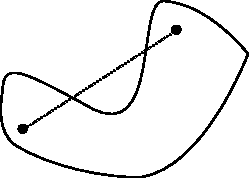
\includegraphics{./images/notConvex.pdf}
\end{center}
\caption{Graphical example for a convex and a nonconvex set}
\label{Fig:convexNotConvex}
\end{figure}

Convex sets have a lot of nice properties. Luckily feasible regions are always convex. This is the main reason why we can efficiently solve LPs.

\begin{Def}[Vertex]\label{Def:Vertex} Let P be a polyhedron. A vector $x\in P$ is a \emph{vertex} of P if there is a $\vec c\in \R^n$
 s.t. $cx\leq cy$ for all $y\in P$ that a different from x; that is $x$ is the minimiser for some cost vector (the unique optimal solution for a LP).
\end{Def}

\begin{Def}[Extreme Point]\label{Def:ExtremePoint} An \emph{extreme point} of a ployhedron P is a vector $x\in P$ s.t. $x$ is not a convex combination of any two vectors $y,z\in P$ different from $x$.
\end{Def}

\begin{Def}[Active Constraint] Let $P$ be a polyhedron that is defined by some linear inequalities $a_i$: $P=\{x|a_ix\geq b_i\}$. We'll say that the $i$-th constraint is \emph{active} at a point $x$ if we have equality there $a_ix = b_i$
\end{Def}

\begin{Def}[Basic Feasible Solution]\label{Def:BFS} Let $P$ be a polyhedron. Then $x\in P$ is a \emph{basic feasible solution} if the set of active constraints has full rank, that is there are $n$ linearly independent active constraint vectors at the point $x$.
\[\mbox{rank}(\{a_i\in \R^n|a_ix=b_i\}) = n\]

In particular there never is a b.f.s. if we have less than $n$ constraints.
\end{Def}

Now we want to prove that the three definitions \ref{Def:Vertex}, \ref{Def:ExtremePoint} and \ref{Def:BFS} all are equivalent to each other.

\begin{thm} Let $P$ be a polyhedron and $x\in P$. The following are equivalent
\begin{enumerate}
\item $x$ is a vertex
\item $x$ is an extreme point
\item $x$ is a basic feasible solution
\end{enumerate}
\end{thm}